% Chapter 3.6: Medical Imaging and Tomographic Reconstruction
% Part III of the book.

\chapter{Medical Imaging and Tomographic Reconstruction}
\label{ch:part3-medical-imaging-and-tomographic-reconstruc}
\label{sec:medical_imaging}
% -----------------------------------------------------------------------------

Tomography is among the oldest inverse problems in scientific computing and, in
current clinical practice, one of the most heavily engineered. A computed tomography
(CT)\index{computed tomography (CT)} scanner does not measure the attenuation
field it is asked to display; it measures line integrals of that field, and the
image is recovered afterwards. When the ray family is dense, recovery is a
well-conditioned quadrature and filtered backprojection (FBP)\index{filtered
backprojection (FBP)} returns an axial slice in milliseconds. When it is not ---
eighteen sampled angles where the geometry supports seven hundred and twenty, or
an angular arc truncated by anatomy well short of the half-turn the geometry
would need --- the same formula returns
streaks\index{streak artifact}. The standard remedies both cost something.
Model-based iterative reconstruction buys consistency with the physics at the
price of tens of forward-and-backward projection passes per slice. Learned
reconstructors buy artifact suppression at the price of a network tied to the
detector and angular geometry it was trained on, so a new protocol is a new
model.

That second price is what Parts~I and II were written to remove. The operator
formulation treats measurement-to-image as a map between function spaces, with
the sampling grid a discretization of the input rather than part of the input's
identity. Section~\ref{sec:ch06-definition} makes ``the same operator on
different grids'' precise, Section~\ref{sec:ch06-zeroshot} states when one
trained network may be served on several, and
\chapref{ch:part2-fourier-neural-operators-fno-from-scratch} supplies the
frequency-indexed weights that make a global spectral map affordable. This
chapter puts the three to work on the Radon transform.

The route is short. Section~\ref{sec:ch36-radon} states the continuous forward
model, the FBP inversion, and what undersampling in angle does to the range of
the sampled operator. Section~\ref{sec:ch36-operators} takes up the two
arrangements by which a learned map has been inserted into that inversion --- an
unrolled cascade that alternates learned refinement with a projection onto the
measured data, aimed at sparse-view data at several sampling rates, and a learned
filtering stage inside FBP itself, aimed at data whose angular range is
truncated --- and keeps them apart, because they answer different defects.
Section~\ref{sec:ch36-metrics} sets out what the image-quality metrics used to
report such reconstructions can and cannot certify, and lists the ways the
pipeline fails quietly. Reconstruction is an inverse problem, so its
characteristic failure is not a divergent iterate but a plausible
image\index{inverse problem!ill-posedness in tomography}.

% -----------------------------------------------------------------------------
\section{The Continuous Inverse Radon Transform}
\label{sec:ch36-radon}
% -----------------------------------------------------------------------------

Let $f \in L^2(\mathbb{R}^2)$ represent the continuous attenuation coefficient
field of patient anatomy, supported inside a field of view of radius $R$. Under
the monochromatic idealization, the forward projection measurement is modeled by
the two-dimensional Radon transform:
\begin{equation}
  \label{eq:ch36-radon}
  p(\theta, s) = (\mathcal{R} f)(\theta, s) = \int_{\mathbb{R}^2} f(x_1, x_2) \, \delta(x_1 \cos\theta + x_2 \sin\theta - s) \, dx_1 dx_2,
\end{equation}
where $\theta \in [0, \pi)$ is the projection angle, $s \in [-R, R]$ is the
detector position, $\delta$ is the Dirac distribution, and
$(\mathcal{R}f)(\theta,s)$ is therefore the integral of $f$ along the line
$x_1\cos\theta + x_2\sin\theta = s$ \index{Radon transform}. The collection of
projections $p(\theta, s)$ forms a two-dimensional \textbf{sinogram}
\index{sinogram}: one axis is angle, the other detector position, and a point of
the object traces a sinusoid through it. The idealization is where the first
model error enters: real beams are polychromatic, so the recorded quantity is
not linear in $f$; scatter adds a smooth positive bias; and where attenuation is
high few photons arrive, so the noise is neither Gaussian nor angle-independent
\index{beam hardening}. A reconstructor trained on exact line integrals inherits
all three as unmodeled shift.

Inversion is classical because the one-dimensional Fourier transform in the
detector variable recovers the two-dimensional spectrum of $f$ line by line:
with $\hat p$ the one-dimensional
transform of $p(\theta,\cdot)$ at frequency $\omega$ and $\hat f$ the
two-dimensional transform of $f$,
\begin{equation}
  \label{eq:ch36-slice}
  \hat{p}(\theta,\omega) = \hat{f}(\omega\cos\theta,\,\omega\sin\theta),
\end{equation}
the \textbf{Fourier slice theorem}\index{Fourier slice theorem} --- each
projection fills one central line of the object's spectrum. Reading
\eqref{eq:ch36-slice} backwards gives FBP:
\begin{equation}
  \label{eq:ch36-fbp}
  f_{\text{FBP}}(x) = \mathcal{R}^* \big( \mathcal{F}^{-1} (|\omega| \cdot \mathcal{F} p) \big)(x),
\end{equation}
where $\mathcal{F}$ and $\mathcal{F}^{-1}$ act in the detector variable,
$|\omega|$ is the ramp filter, and $\mathcal{R}^*$ is the adjoint of the Radon
transform, which smears each filtered profile back along the rays that produced
it. Two consequences decide this chapter. Exactness requires the polar sampling
of \eqref{eq:ch36-slice} to fill the Fourier plane at the density the
reconstruction grid demands: complete angular coverage, and detector spacing
below the Nyquist rate for
the target pixel size. And the ramp is a positive-order operator --- it gains
one derivative --- so it amplifies high-frequency noise exactly where the
measured signal is weakest. Dose and resolution are traded through the same
factor, which is why dose reduction cannot be handled by filtering alone.

In sparse-view CT, the sinogram is sampled at only $M \ll M_{\text{Nyq}}$ angles
(e.g., $M = 18$ or $36$ views instead of $720$), where $M_{\text{Nyq}}$ is the
count at which the angular step $\pi/M$ falls below the ratio of the detector
pitch to the field-of-view radius --- the spacing at which two neighboring views
displace the object by less than one detector element at the edge of the field.
Inverting the sampled operator
becomes a severely ill-posed inverse problem \cite{stuart2010inverse}. Write
$\mathcal{A} = \mathbf{M}\mathcal{R}$ for the continuous transform composed with
the restriction $\mathbf{M}$ to the $M$ measured angles; $\mathbf{M}$ is where
the protocol lives. For any finite angle set $\mathcal{A}$ has an
infinite-dimensional null space in $L^2(\mathbb{R}^2)$, since any field whose
integral vanishes along every measured ray is invisible to the data. FBP of
sparse data is thus not an approximate inverse of $\mathcal{A}$ but the exact
inverse of an operator whose input the scanner never delivered, with the
unwritten Fourier lines set to zero. In heuristic terms, each unmeasured
direction of integration leaves the structure along it unconstrained, and the
ramp filter turns that unconstrained content into lines of discontinuity
radiating from high-contrast objects. The result is the artifact the classical
recipe is known for: intense streaks, high noise, and blurred organ boundaries.
Figure~\ref{fig:vol3_ct} draws the geometry that produces this: sources and
detectors at a set of angles around the object, and the gaps between them are the angles never
measured. The conclusion it supports is structural and narrow. Each unmeasured direction is a
degree of freedom the data never constrains, and the ramp filter is what turns that
unconstrained content into the streaks the classical recipe is known for. Nothing on the plate
bears on accuracy --- that is the question of Section~\ref{sec:ch36-metrics} --- and no
reconstruction, phantom, Hounsfield value or error figure is drawn here or should be read off
it.

\begin{figure}[htbp]
\centering
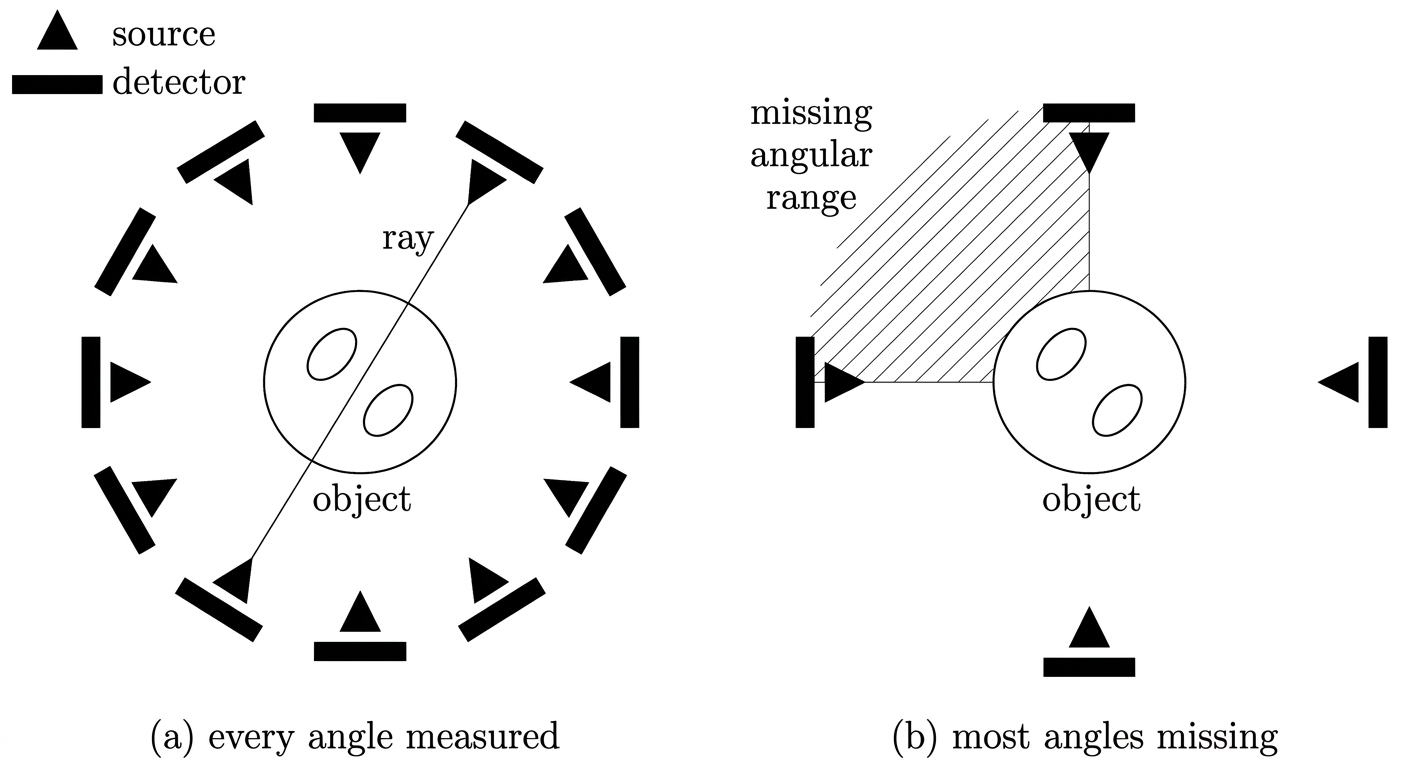
\includegraphics[width=0.92\textwidth]{fig_ct_geometry.png}
\caption{\textbf{Sparse-view acquisition geometry, as a two-panel schematic.} A source is drawn as a
filled triangle and its opposing detector as a thick bar, identified once by a legend rather than by
arrows aimed at the ring. Panel~(a): twelve source-detector pairs spaced all the way round the object,
with one ray drawn plainly through it --- every angle measured. Panel~(b): four pairs, at top, right,
bottom and left, and the hatched wedge is the angular range no view ever crosses --- most angles
missing. The contrast between the panels is the whole content, and it is the contrast
\eqref{eq:ch36-slice} turns into a null space: what is not sampled is not recovered. The plate shows
no phantom reconstruction, no Hounsfield value and no error figure; quantitative claims belong to the
text and its citations, not to this figure.}
\label{fig:vol3_ct}
\end{figure}

How the data fail matters as much as how sparse they are, and the two
arrangements of the next section attach to one failure each. Sparse-view
acquisition is a \emph{density} failure: the angular range is complete, the
samples inside it are too few, and adding views at finer spacing repairs the
defect in the limit. Limited-angle acquisition is a \emph{coverage} failure: an
arc is absent, no number of extra views inside the measured arc recovers it, and
the null space contains smooth anisotropic structure --- the kind of content a
prior is most willing to invent. One geometric fact governs both. The sinogram
is periodic in one coordinate and not the other: $\theta$ closes on itself
modulo the identification $p(\theta+\pi,-s) = p(\theta,s)$, while $s$ is a
finite interval across which nothing repeats. A spectral treatment of the
sinogram tensor must therefore choose which axis carries the Fourier structure,
and a multiplier applied along $s$ silently imposes a wraparound boundary
condition no patient satisfies. That choice, not the depth of the network, is
what separates a tomographic operator from a stock two-dimensional spectral
model.

% -----------------------------------------------------------------------------
\section{Two Operator-Learning Arrangements}
\label{sec:ch36-operators}
% -----------------------------------------------------------------------------

Two arrangements introduce continuous neural operators into this pipeline, and
the inherited record presents them as one family. They are not. The first
targets sparse-view data at \emph{several} sampling rates
\index{sparse-view CT}. It rests on two claims, and the property they buy
together is of exactly the kind Part~I's discretization-invariance machinery was
built to state. The first claim is a dual-domain design: the network acts in
sinogram space and in image space, where an artifact localized in one is spread
across the other \index{dual-domain reconstruction}. The second is that its
convolution kernels are parameterized as functions on the continuum and evaluated
on whatever grid the data arrive on, so that the parameters are decoupled from
the detector sampling density; the same parameterization is additionally made
equivariant to the rotations the tomographic geometry acts with, the rotational
structure the previous section located in the angle axis
\index{rotation equivariance}\index{resolution-agnostic operator!see also
discretization invariance}. The consequence is the property such a model is built
for: one trained network reconstructs data acquired at different angular and
detector rates without retraining. Whether it is \emph{accurate} at a rate it was
never trained on is the separate question Section~\ref{sec:ch36-metrics} returns
to, and the two shifts a device serving many protocols must actually survive ---
a change of dataset, a change of noise level --- are measured rather than granted
by the parameterization. Inference in this arrangement is an unrolled
cascade alternating sinogram-domain operator refinement, projection-data
consistency updates with $\mathcal{A} = \mathbf{M}\mathcal{R}$, and image-space
operator denoising. Displayed in the form such steps usually take, the
consistency update is
\begin{equation}
  \label{eq:ch36-consistency}
  u^{(j+1)} = u^{(j)} - \gamma_j\, \mathcal{A}^{*}\big(\mathcal{A} u^{(j)} - p_\delta\big), \qquad \mathcal{A} = \mathbf{M}\mathcal{R},
\end{equation}
with $p_\delta$ the measured noisy sinogram, $\mathcal{A}^*$ the adjoint of the
sampled forward operator, and $\gamma_j$ a step size; in the unrolled setting
$\gamma_j$ and the surrounding refinements are learned rather than chosen, and
the fixed projection becomes a learned operator applied a fixed number of
times \index{data-consistency projection}.

The second arrangement addresses the other defect: \emph{limited-angle}
tomography, in which an arc of the acquisition is simply absent
\index{limited-angle tomography}. Its posture is the opposite of an unrolled
cascade, and its substitution is a single one: a Fourier
neural operator (FNO)\index{Fourier neural operator (FNO)!in reconstruction} in
the sense of \cite{li2021fourier} is inserted into the filtering stage of FBP
itself, so the
analytic structure of \eqref{eq:ch36-fbp} is retained and the learned component
is confined to extrapolating the sinogram into the unmeasured angular region
before backprojection. The extrapolation is not free-form; it is constrained by
the \emph{moment conditions}, the family of identities
\begin{equation}
  \label{eq:ch36-moment}
  m_k(\theta) \;=\; \int_{\mathbb{R}} s^{k}\, p(\theta,s)\, ds \;=\; \int_{\mathbb{R}^2} f(x)\,\big(x_1\cos\theta + x_2\sin\theta\big)^{k}\, dx, \qquad k = 0,1,2,\ldots.
\end{equation}
The second equality is \eqref{eq:ch36-radon} tested against $s^k$. Its content is
that for data which are the projection of \emph{some} attenuation field, the
right-hand side is a homogeneous polynomial of degree $k$ in
$(\cos\theta,\sin\theta)$
\index{moment conditions (range conditions)!Helgason--Ludwig type}. Total mass,
center of mass, and the second moments of $f$ are read off $m_0$, $m_1$, $m_2$,
so an extrapolation preserving these low-order moments cannot add or relocate
mass: it stays inside the range of the continuous transform up to the order at
which the conditions are imposed. That is the whole content of the instruction
to enforce moment conditions, and it is why the arrangement is defensible on real
incomplete data rather than merely fitted to them. Two consequences follow from
keeping the analytic pieces analytic. The first is a cost accounting in the
console's own units: this arrangement inserts one learned completion of the
sinogram into a pipeline whose projection pass it does not touch, whereas an
unrolled cascade changes what the console has to run and must be priced from
scratch. Whether a learned filtering stage in fact executes at FBP's cost on a
given scanner is a measurement this book does not have, and it is not a
comparison the arrangement's structure settles. The second is that the residual
of \eqref{eq:ch36-consistency} remains available as a check on the completed
data: the extrapolated wedge can be reprojected and tested against the measured
rays without a reference image in hand, which is the check
Section~\ref{sec:ch36-metrics} returns to.

Table~\ref{tab:ch36-operators} sets the two side by side, and the row to read
is the fourth. The cascade's commitment is on sampling \emph{density}, precisely
the variable Part~I's definition of discretization invariance governs; the
learned filtering stage's is on angular \emph{coverage}, which is not a
discretization of anything but a property of the geometry, and no
resolution-agnostic parameterization removes it. The final row is the editorial
accounting: the inherited record attaches accuracy and runtime gains to specific
reconstructors, and this book carries none of them, because a margin is a
statement about the model it was measured on. The consequences for how such a
margin should be read are Section~\ref{sec:ch36-metrics}.

\begin{table}[htbp]
\centering
\small
\caption{\textbf{Two operator reconstructions, two defects.} The two arrangements of Section~\ref{sec:ch36-operators} as this book formulates them. The discretization row is this book's reading of what each arrangement commits to; the other rows state where the learning sits and what is left analytic. No accuracy or runtime figure is carried: the measurements in the inherited record belong to reconstructors this book does not name, and Section~\ref{sec:ch36-metrics} explains why a margin quoted against untuned filtered backprojection is not a margin against the classical recipe.}
\label{tab:ch36-operators}
\resizebox{\textwidth}{!}{%
\begin{tabular}{lll}
\toprule
 & \textbf{Unrolled cascade} & \textbf{Learned filtering stage} \\
\midrule
Defect addressed & Sparse view: too few angles, full arc & Limited angle: arc missing entirely \\
Where learning acts & Sinogram and image domains, alternated & Sinogram extrapolation inside FBP \\
What stays analytic & Projection $\mathbf{M}$, Radon $\mathcal{R}$ in \eqref{eq:ch36-consistency} & Ramp filter and backprojection $\mathcal{R}^*$ in \eqref{eq:ch36-fbp} \\
Discretization commitment & Detector and view density, deliberately removed & Angular range, deliberately retained \\
Figures certified here & None; multi-rate gains unmeasured & None; cost relative to FBP unmeasured \\
\bottomrule
\end{tabular}%
}
\end{table}

% -----------------------------------------------------------------------------
\section{Reported Accuracy, Error Accounting, and Failure Modes}
\label{sec:ch36-metrics}
% -----------------------------------------------------------------------------

Reconstructions of this kind are reported in three quantities, all of them
computed against a reference image $f$ --- a full-dose or simulated
reconstruction that the low-dose protocol being evaluated does not itself possess
--- on a display window with peak level $L$. With $u$ the reconstruction and
$\Omega$ the field of view,
\begin{equation}
  \label{eq:ch36-metrics}
  \begin{aligned}
    \mathrm{RMSE}(u,f) & = \Big( \tfrac{1}{|\Omega|}\int_{\Omega} \big(u(x)-f(x)\big)^{2}\,\mathrm{d}x \Big)^{1/2}, \\[2pt]
    \mathrm{PSNR}(u,f) & = 10\log_{10}\!\big( L^{2}/\mathrm{RMSE}(u,f)^{2} \big),
  \end{aligned}
\end{equation}
where the root-mean-square error (RMSE)\index{root-mean-square error (RMSE)} is
taken in Hounsfield units and the peak signal-to-noise ratio
(PSNR)\index{peak signal-to-noise ratio (PSNR)} is its logarithmic rescaling; the
third quantity, the structural similarity index measure
(SSIM)\index{structural similarity index measure (SSIM)}, compares local
luminance, contrast and structure between $u$ and $f$ over a sliding window. The
operating points the inherited record attaches to an abdominal and kidney CT
benchmark at $18$ projection views are not reproduced here. They were measured on
reconstructors this book does not name; a point on a curve and an average over
sampling rates are different objects, and the record mixed the two; and the
baseline they were quoted against is not the classical recipe but one
parameterization of it. That last defect is independent of which network sits on
the other side of the comparison. A baseline whose RMSE spans the whole
soft-tissue band marks itself as an FBP of the raw sparse data rather than a
tuned one: at $18$ views a console runs
an apodizing window and an object mask, each trading resolution for the very
streak suppression the comparison is meant to win, and the fair comparator at
low view count is a regularized iterative reconstruction. ``Outperforming
classical FBP'' is thus a statement about one parameterization of a method.

Of the three quantities in \eqref{eq:ch36-metrics}, only RMSE is interpretable
without further
convention. The Hounsfield unit (HU)\index{Hounsfield unit (HU)} is the
calibrated attenuation scale $\mathrm{HU}=1000(\mu-\mu_{\text{water}})/\mu_{\text{water}}$,
with air near $-1000$, water at $0$, and cortical bone well above
$+1000$. An RMSE of a few tens of HU is an absolute attenuation error of a few
percent of the water-to-bone span, and of the same order as the contrast between
a focal lesion and the parenchyma around it. The honest reading of an error at
that magnitude is less
flattering than a decibel figure sounds: the reconstruction is accurate to
within the contrast it must display --- a claim about detectability at the edge
of the range, not about recovery.
PSNR is a logarithm relative to the assumed peak $L$ of
\eqref{eq:ch36-metrics}, and the peak convention
--- window, level, clipping --- moves it by several dB at fixed error, so a dB
figure without its convention does not compare across papers.
SSIM rewards smoothness, so an over-smoothing network can
beat a sharper one while destroying the low-contrast features the dose reduction
existed to preserve, and it is full-reference: the ground truth a low-dose
protocol lacks is borrowed from a full-dose or simulated scan, itself a
reconstruction with its own kernel. Task-based evaluation --- lesion detection
scored by an observer study or a model observer --- is what a radiologist
consumes, and no reconstruction discussed here is verified against it in this
book
\index{task-based image quality assessment|textbf}.

Error accounting says why better metrics will not close that gap. Decompose the
reconstruction error orthogonally in $L^2(\mathbb{R}^2)$ against the null space of
the sampled operator:
\begin{equation}
  \label{eq:ch36-error}
  \hat f - f \;=\; \Pi_{\mathcal{N}(\mathcal{A})}\big(\hat f - f\big) \;+\; \big(I - \Pi_{\mathcal{N}(\mathcal{A})}\big)\big(\hat f - f\big),
\end{equation}
with $\hat f$ the reconstruction, $f$ the truth, $\mathcal{A}=\mathbf{M}\mathcal{R}$
as before, and $\Pi_{\mathcal{N}(\mathcal{A})}$ the orthogonal projector onto
$\mathcal{N}(\mathcal{A})$ \index{null space!of the sampled measurement
operator}\index{error decomposition!in tomographic reconstruction}. The identity
is the argument. A reconstruction exactly consistent with the measured data puts
all of its error in the first term, where the measurement at hand cannot find
it; that term is set by the learned prior, not by the physics.
Which term dominates is regime-dependent: at $18$ views the null-space term
governs and the image is prior-driven; at full sampling with low dose the second
governs, and what matters is noise propagation and the consistency residual in
\eqref{eq:ch36-consistency}. Across protocols a third error binds, outside
\eqref{eq:ch36-error} because that split holds the operator fixed: the
approximation and discretization error that attaches to the discretization-invariant
formulation \cite{kovachki2023neural}, bounded in this book as \eqref{eq:ch06-rate}
under a compactness hypothesis on the training support --- the discretization leg
of \eqref{eq:ch06-decomp} \cite{subedi2024controlling}. The
caveat of
Section~\ref{sec:ch06-zeroshot} bites harder here than anywhere in the book:
moving one model to a finer grid is resolution \emph{transfer}, not recovery of
detail the sampling destroyed, and in sparse-view acquisition that detail is
genuinely gone --- which is why the moment conditions of
\eqref{eq:ch36-moment} constrain the extrapolation rather than supply content.

Two verification consequences follow. Held-out error on the training
distribution scores a network on the prior it was trained to use, so the checks
that bite move the protocol: train at high view count and serve at low, train on
one dataset and test on another, inject sinogram noise and watch the image
metrics and the HU bias separate. The cheaper check needs no ground truth at all:
reproject the reconstruction with $\mathcal{A}$ and compare against the measured
$p_\delta$, so that a large residual becomes the refusal the deployed-surrogate
test of \chapref{ch:part2-production-deployment-and-high-throughput-} asks for
but cannot supply, needing held-out labels where this check does not
\index{verification!consistency check at inference}. The failure modes are then
predictable. Streak suppression and lesion restoration act on the same degrees
of freedom, so the boundary recovered in box~B of
Figure~\ref{fig:vol3_ct} is an inference, and the only defensible safety statement
about it is conditional on the training distribution. HU error is not cosmetic:
treatment-planning systems convert HU into electron density, so a bias of tens of
units propagates into whatever the next device computes. Data are the binding
constraint: paired low-dose and reference scans are expensive, and the reference
carries its own kernel. Clinical reconstruction software is also
regulated as a medical device, cleared against a predicate device's output --- a
harder comparison when the noise texture varies with the anatomy, since the two
images are then not two renderings of one measurement.
Prospective multi-center validation on diverse cohorts is the roadblock named in
\chapref{ch:part3-synthesis-matrix-and-real-world-deployment};
``resolution-agnostic'' describes a model's parameterization, not a waiver of
per-protocol verification \index{medical device
regulation!of reconstruction software}.

% -----------------------------------------------------------------------------
% Bridge to Chapter 3.7
% -----------------------------------------------------------------------------
\medskip
Every reconstruction above is an arrangement of two kinds of constraint. The
moment conditions \eqref{eq:ch36-moment} are hard in the strong sense: an
extrapolation that satisfies them does so whatever the weights happen to be,
because the admissible set is built into the computation rather than asked of
it. The projection step \eqref{eq:ch36-consistency} is hard in a weaker sense
easy to lose: $\mathcal{A}$ and $\mathcal{A}^*$ there are the analytic
operator and its adjoint, unlearned even where $\gamma_j$ is not.
The learned prior is soft: it holds in expectation, at a weight
chosen during training, and it is exactly where the null-space term of
\eqref{eq:ch36-error} lives. Stripped of tomography, that opposition is the
subject of \chapref{ch:part3-boundary-condition-enforcement-neural-oper}.
Classical solvers impose boundary data by construction --- Dirichlet conditions
carried by the test space $v \in H^1_0(\Omega)$ in the finite element method,
local flux balance across cell interfaces in the finite volume method,
boundary-conforming bases in a spectral discretization
--- whereas a neural operator's global convolution satisfies none of them by
default, and the field-of-view edge, the object's support, and the periodicity of
the angle axis are boundary conditions in disguise. The next chapter compares
the two remedies: a distance envelope that attains the
boundary value for every parameter vector, and a penalized boundary residual in
the loss. This chapter has priced that distinction from the other side. In
tomography the hard constraint costs one reprojection and the soft one carries
the entire error budget --- a ratio worth knowing before the choice is made for
a partial differential equation\index{boundary condition!hard versus soft
enforcement}.
